\section{Performance Evaluation}

Eine Audio-Plugin läuft in einer Umgebung mit vielen anderen Komponenten mit dem es CPU-Ressourcen teilt. Verarbeitung von Audiodaten muss innerhalb diskreten Zeitintervallen von der Audio-Hardware bestimmt und einige Einstellung der Benutzer zu konfigurieren abgeschlossen werden kann. Typische Audio-Sampling-Frequenzen 44,1 kHz, 48 kHz, 88,2 kHz und 96 kHz. Mit 44,1 kHz als Beispiel bedeutet dies, daß die für eine einzelne Probe erforderlichen Berechnungen innerhalb von 0,023 ms durchgeführt werden. Interrupts würde von der Audio-Hardware in Abständen von 0.023ms als auch empfangen werden, und dies würde auf dem Betriebssystem der CPU wenn zu viel von einem belasten. Stattdessen werden Anträge für neue Audiodaten in Puffern von Proben gebündelt. Die Größe der Puffer ist ein Parameter, der Benutzer zu ändern, es in der Regel bei 512 Proben festgelegt, kann aber so günstig wie 16 Proben sein.

Increasing the buffer size, increases the amount of time that the CPU has to provide the audio data to the audio hardware, this introduces latency into the system though. A buffer size of 512 samples equates to a latency of 11.60ms. A 16 sample buffer size equates to 0.36ms.

If a single plugin requires 1.0ms to complete its processing then it will not finish in time if the buffer size is set too low. If the buffer size is just high enough, then there still might not be enough CPU resources left for other plugins to complete their tasks.

\subsection{Synchronous Performance}

This project offloads the processing to an external SBC device. However, no resources are saved if the audio plugin is blocked while it waits for the results from the SBC device. Since the external SBC devices are slower than the main CPU, the processing time will take longer. Adding the time it takes to serialise and deserialise the Datagram packet at each end will degrade performance even more.

Figure~\ref{fig:local_vs_remote} illustrates the problem in more detail.

\begin{figure}[H]
    \centering
    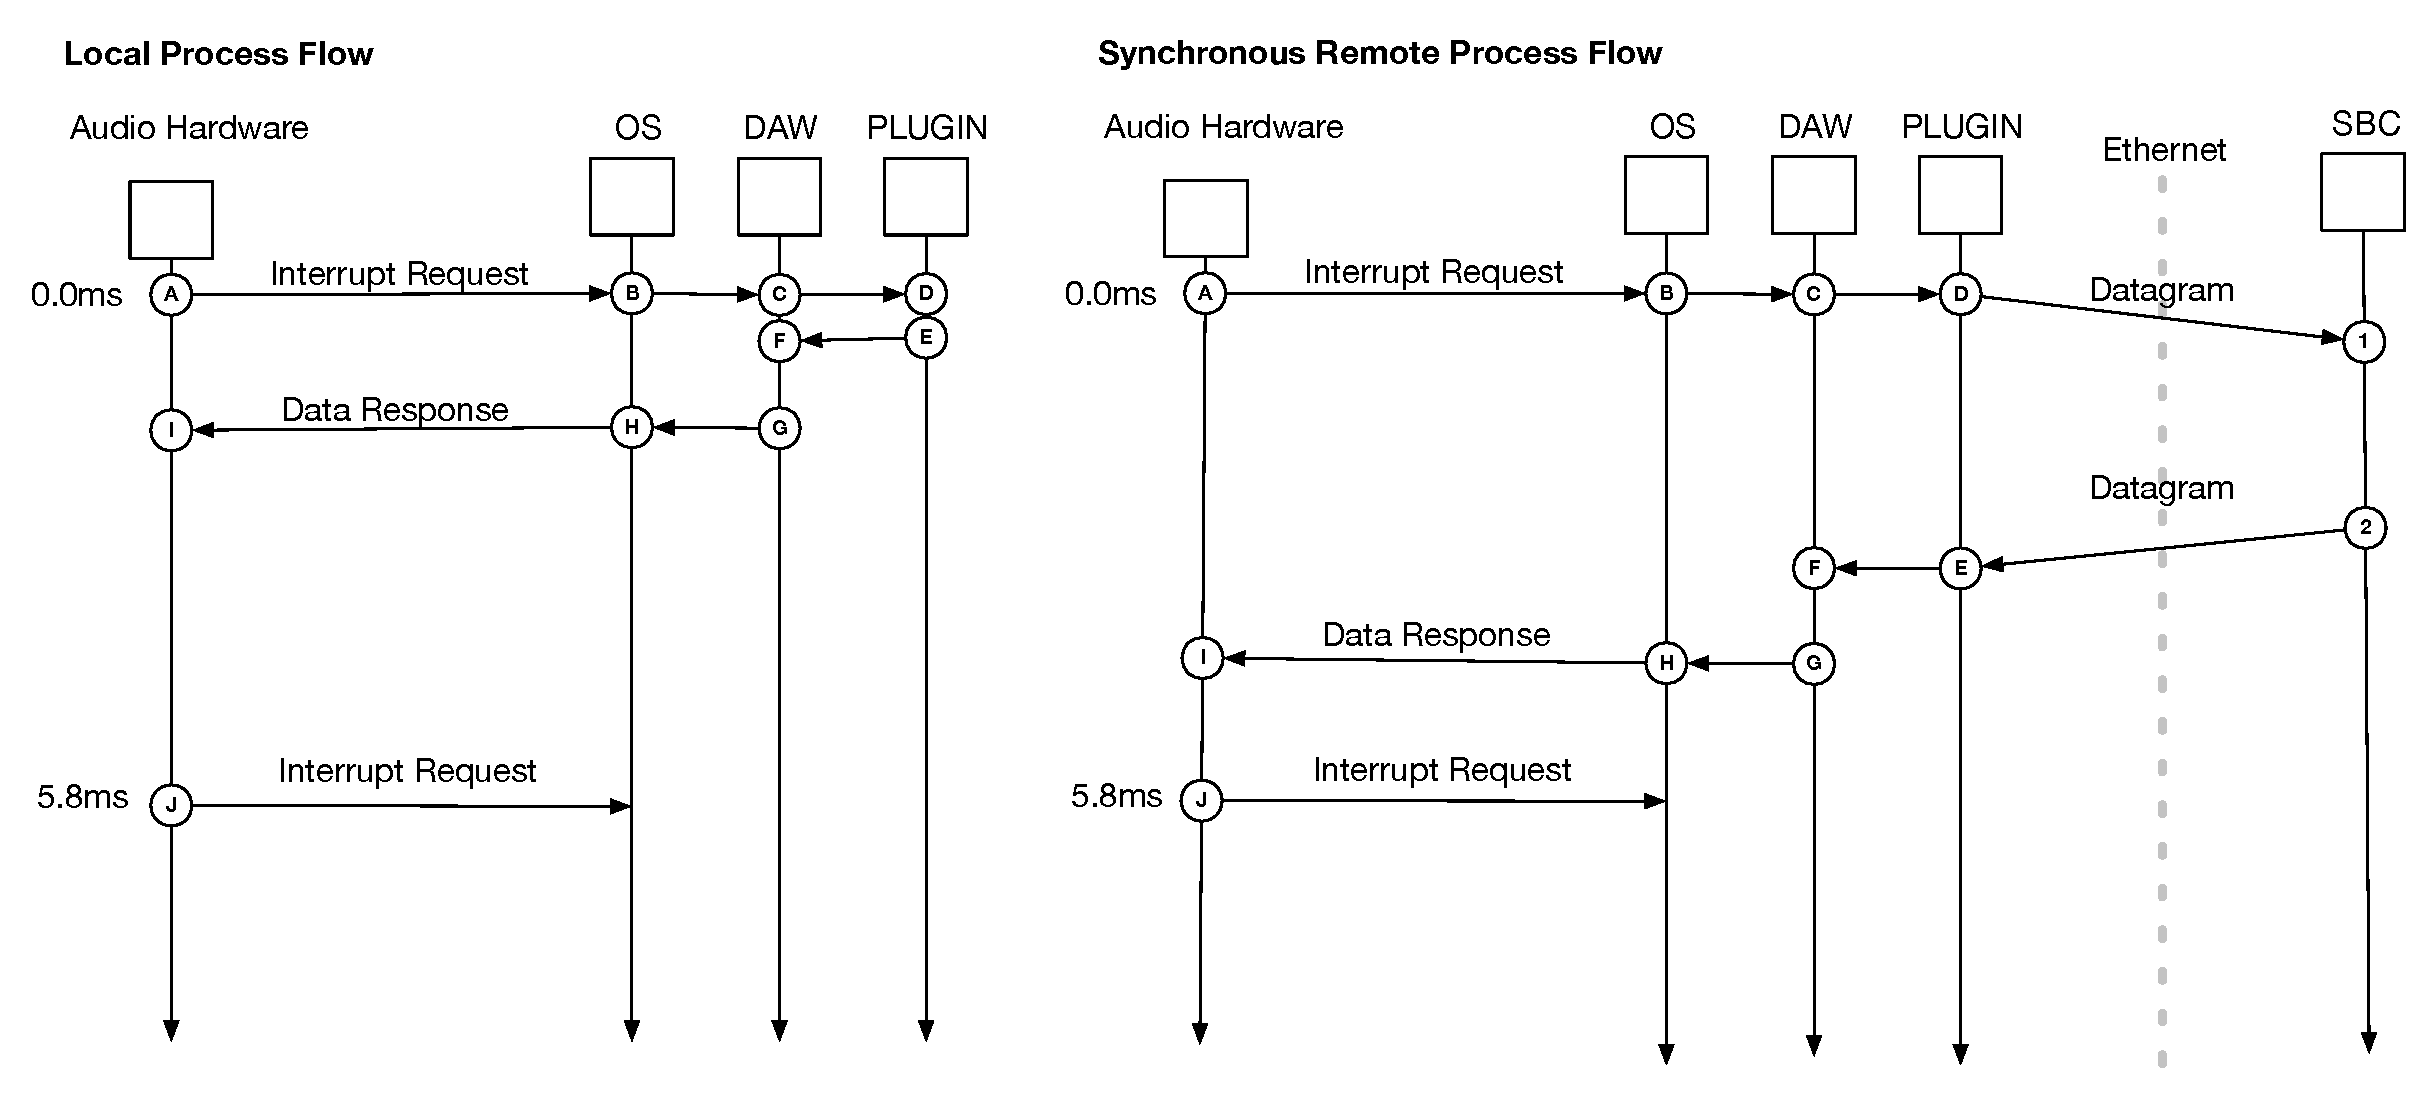
\includegraphics[width=\textwidth]{assets/conclusion/process_flow_compared.pdf}
    \caption{Local vs Remote Synchronous Processing}
    \label{fig:local_vs_remote}
\end{figure}

The example shows the audio hardware polling the operating system in intervals of 5.8 ms. This corresponds to a buffer size of 256 samples. The time interval between states D and E represents the time it takes for a plugin to process a buffer of 256 sample. The DAW can perform other audio processing functions ( including passing the buffer to other plugins ) in the interval between F and G. After states G and H the DAW and OS are free to be able to do other things, like update the GUI or check for email.

With synchronous remote processing the time between states 1 and 2 in the Remote Process Flow will add directly to the time between D and E. If that time is significantly higher than the local processing then the ability of the DAW and the OS to perform other critical tasks is impaired.

\begin{table}[H]
\begin{center}
\begin{tabular}{ |p{1.4cm}||p{1.5cm}|p{1.7cm}|p{1.7cm}|p{1.6cm}|p{1.4cm}|  }
 \hline
 puffergrösse    & pufferzeit (ms)    & rtTime (ms)   & pTime (ms)    & tTime (ms) & \% von pufferzeit\\
 \hline
 64             & 1.451247      & 0.574672          & 0.015857          & 0.558815      & 39.59 \\
 96             & 2.176870      & 0.575419          & 0.015851          & 0.559568      & 26.43 \\
 128            & 2.902494      & 0.59001           & 0.016519          & 0.573491      & 20.32 \\
 192            & 4.353741      & 0.67902           & 0.019013          & 0.660007      & 15.59 \\
 256            & 5.804988      & 0.707267          & 0.020352          & 0.686915      & 12.18 \\
 512            & 11.60997      & 0.707905          & 0.026348          & 0.681557      & 6.097 \\
 \hline
\end{tabular}
\end{center}
\caption{Measured Times for Synchronous Processing}
\label{tab:latency_comp}
\end{table}

Table~\ref{tab:latency_comp} shows the measured times for various buffer sizes in a remote synchronous environment that does no actually audio processing. An audio system running with a buffer size of 64 samples has 1.451ms to complete all tasks and provide the audio hardware with the resulting buffer. "rtTime" is the total round trip time. This corresponds to the time between states D and E of the Synchronous Remote Process Flow diagram in Figure~\ref{fig:local_vs_remote}. "pTime" is time interval between states 1 and 2 on the SBC device, the time spent processing the data. In this case there was no processing so this is only the measures the time spent deserialiseing and serialising the datagrams into audio and midi data. "tTime" is the "rtTime" subtracted by the "pTime" and is the packaging overhead required to send and receive data from the SBC device.

The last column, "\% of limit", shows how much time was spent in total as a percentage of the limit. At a buffer size of 64 samples 39.59\% percent of the total time available was spent by a single plugin. This does not leave much time for other processes on the CPU. For a buffer size of 512 samples the "\% of limit" value is much lower. The total system latency is slightly higher that the stated 10ms maximum though, and the synchronous design has not reduced the processing load on the CPU at all.


\subsection{Asynchronous Performance}

Instead of waiting for a response from the SBC device as in the synchronous method described above the asyncronous method checks if a response is available, if so process it, if not immediately return. The initial request for audio data would return empty, but by the time the second buffer is requested, the first respose from the SBC device might have returned. In both cases the only time spent by the audio plugin itself is the time is takes to serialise and send the data, and to receive and deserialise the data. These are the intervals between the states D and E and M and N represented in figure~\ref{fig:async_remote}.

\begin{figure}[H]
    \centering
    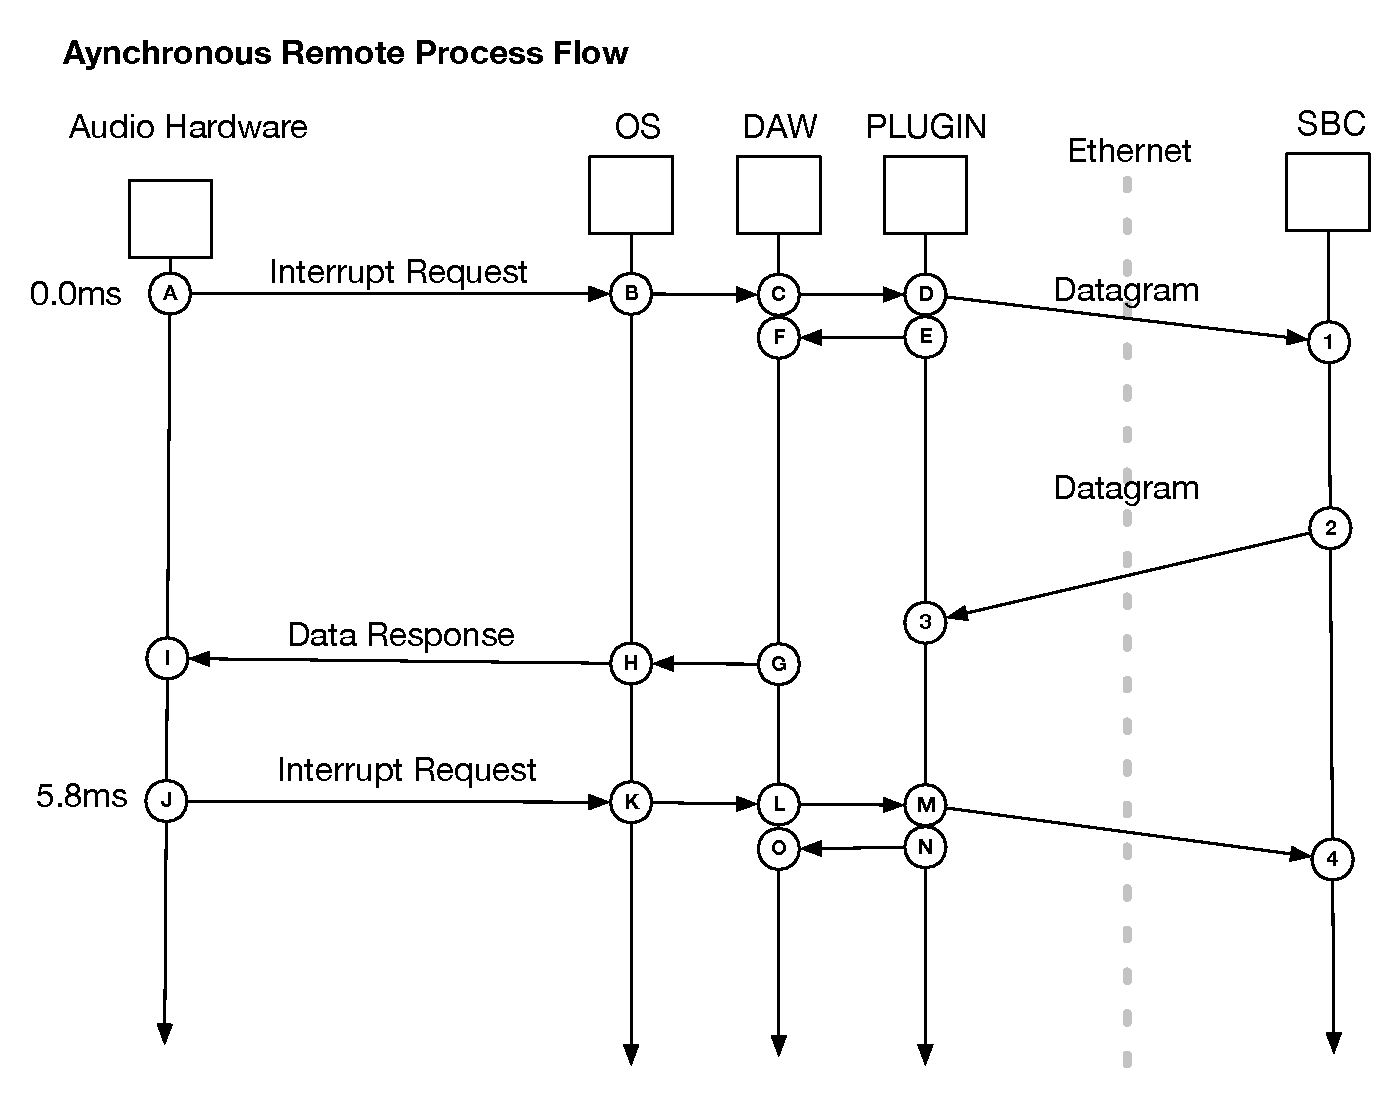
\includegraphics[width=\textwidth]{assets/conclusion/async_flow.pdf}
    \caption{Local vs Remote Synchronous Processing}
    \label{fig:async_remote}
\end{figure}

By the time the second cycle begins (J in figure~\ref{fig:async_remote}) processed data from the first cycle has returned. The time between events M and N is no longer proportional to the amount of time needed to actuall process the data, only to the time it takes to prepare the data for sending and receiving. Table~\ref{tab:latency_async} shows the measured times.

\begin{table}[H]
\begin{center}
\begin{tabular}{ |p{1.4cm}||p{1.5cm}|p{1.7cm}|p{1.7cm}|p{1.6cm}|p{1.4cm}|  }
 \hline
 puffergrösse    & pufferzeit (ms)    & rtTime (ms)   & pTime (ms)    & tTime (ms) & \% von pufferzeit\\
 \hline
 64             & 1.451247      & 0.031683          & 0.015633          & 0.016050      & 2.18 \\
 96             & 2.176870      & 0.046585          & 0.016076          & 0.030509      & 2.14 \\
 128            & 2.902494      & 0.034745          & 0.016712          & 0.018032      & 1.19 \\
 192            & 4.353741      & 0.052279          & 0.018800          & 0.033478      & 1.20 \\
 256            & 5.804988      & 0.065752          & 0.019646          & 0.046105      & 1.13 \\
 512            & 11.60997      & 0.062939          & 0.019708          & 0.043230      & 0.54 \\
 \hline
\end{tabular}
\end{center}
\caption{Für asynchrone Datenverarbeitung gemessene Zeiten}
\label{tab:latency_async}
\end{table}



In the table above "rtTime" is no longer the actual round trip total processing time, but the "fake" one. Since data is already available at the time the interrupt request is triggered, the plugin can return it's data immediately. This comes at the cost of a delay equal to one interrupt cycle, but the user can set the audio system's buffer size low enough that this is well below the 10ms limit, without needing to use more than 1.2\% of the processing time available.

The asynchronous method brings a real benefit to distributed processing in terms of lighting the load on the CPU. The price of the benefit though is an increase in the latency of the plugin. The processed audio data is always one delayed by one buffer. Another disadvantage is that if several distributed processors are chained in series, as is the case in the demo appliation created for this project, then the latency is cumulative. This results in a total latency that is the limit time multiplied by the number of processors in the plugin.

\subsection{Optimisation Potential}

Several aspects of the application could be optimised to achieve higher performance and lower the latency times.

\subsubsection{Redundancy Reduction}

There are two areas of the application where unnecessary operations are performed and could be optimized. The first is the deserializsation of data when it is returned from the SBC. If serveral networked processes are chained in series, then the returned DiauproMessage could be sent directly to the following process without unnecessarily deserialising and the reserialising the data in between steps. This would be a relatively simple optimization to implement.

The second optimisation is similar but more complicated to implement. In a chain to processes the data would not need to be returned to the master plugin between each step, instead it could be sent to the next node directly. If the next node is located on the same SBC device then an additional hop over ethernet could be skipped as well. In addition serialisation steps between nodes could also be skipped if the nodes performed the operations directly on the data in the DiauproMessage. For this the DiauproMessage would need to be extended to include routing information so that each node knows the next destination point.

Although more complex, the second optimization would have the added benefit that the latency would no longer be a multiple of the full cycle time between interrupt calls. The final data could be gathered after a single cycle.


